%% 4. 「技術研究報告」
\documentclass[technicalreport]{ieicej}
\usepackage[dvipdfmx]{graphicx,xcolor}
%%\usepackage[dvips]{graphicx}
\usepackage[fleqn]{amsmath}
%\usepackage{amsthm}
\usepackage{newtxtext}% 英数字フォントの設定を変更しないでください
\usepackage[varg]{newtxmath}% % 英数字フォントの設定を変更しないでください
\usepackage{wrapfig}
%\usepackage{amssymb}
%\usepackage{bm}

\usepackage{booktabs} %表の線
\usepackage{multirow}
\usepackage{float}
\usepackage{algorithm} %アルゴリズム
\usepackage{algorithmic} %アルゴリズム

\usepackage[legacycolonsymbols]{mathtools}

\tecrepyear{2025}% X を適宜書き換えてください
\jtitle{離散制御器合成における計算空間爆発抑制のための\\段階的なLTSの最小化}
\etitle{Stepwise LTS Minimization to Suppress State Space Explosion \\in Discrete Controller Synthesis}
\authorlist{%
 \authorentry{山口 友輝}{Tomoki Yamaguchi}{T-Tech1}\MembershipNumber{}
 \authorentry{山内 拓人}{Takuto Yamauchi}{WASEDA1}\MembershipNumber{}
 \authorentry{平野 貴規}{Takanori Hirano}{WASEDA2}\MembershipNumber{}
 \authorentry{鄭 顕志}{Kenji Tei}{T-Tech2}\MembershipNumber{}
 %\authorentry{和文著者名}{英文著者名}{所属ラベル}\MembershipNumber{}
 %\authorentry[メールアドレス]{和文著者名}{英文著者名}{所属ラベル}\MembershipNumber{}
 %\authorentry{和文著者名}{英文著者名}{所属ラベル}[現在の所属ラベル]\MembershipNumber{}
}
\affiliate[T-Tech1]{東京科学大学, 〒152–8552 東京都目黒区大岡山 2-12–1}{Institute of Science Tokyo, 2–12–1 Ookayama, Meguro-ku, Tokyo, 152–8552}
\affiliate[WASEDA1]{早稲田大学, 〒162–0042 東京都新宿区早稲田町27 GCS研究機構}{Waseda University, GCS Research and Development Center, Wasedamachi–27, Shinjuku-ku, Tokyo, 162–0042}
\affiliate[WASEDA2]{早稲田大学, 〒162–0042 東京都新宿区早稲田町27 GCS研究機構}{Waseda University, GCS Research and Development Center, Wasedamachi–27, Shinjuku-ku, Tokyo, 162–0042}
\affiliate[T-Tech2]{東京科学大学, 〒152–8552 東京都目黒区大岡山 2-12–1}{Institute of Science Tokyo, 2–12–1 Ookayama, Meguro-ku, Tokyo, 152–8552}

\MailAddress{
$\dagger$yamaguchi.t.a709@m.isct.ac.jp,
$\dagger\dagger$takuto.yamauchi@aoni.waseda.jp,
$\dagger\dagger\dagger$cincischio@ruri.waseda.jp,
$\dagger\dagger\dagger\dagger$tei@comp.isct.ac.jp
}

%\MailAddress{$\dagger$hanako@denshi.ac.jp,
% $\dagger\dagger$\{taro,jiro\}@jouhou.co.jp}

\begin{document}
\begin{jabstract}
%和文あらまし
ある動作環境下において安全性が保証された動作仕様を自動合成する技術として，離散制御器合成に関する研究が進められてきた．しかし，離散制御器合成には，計算空間が指数関数的に増加する課題があった．そこで，本論文では，計算空間削減を目指し，LTSの等価性に基づく最小化を活用した合成手法を提案する．LTSの等価性とは，同じ事象列を再現できるLTS同士を等価とみなす性質であり，この性質を使えば，各段階の離散制御器合成において，LTSを等価で最小なものに変換できる．これを離散制御器合成に導入し，計算空間削減を実現する．
\end{jabstract}
\begin{jkeyword}
%和文キーワード
離散制御器合成，ラベル付き遷移システム，安全性保証
\end{jkeyword}
\begin{eabstract}
%英文アブストラクト
Research on discrete controller synthesis has been conducted as a technique for automatically synthesizing behavior specifications that guarantee safety under a given operating environment. However, discrete controller synthesis suffers from the problem of exponential growth in the state space. In this paper, we propose a synthesis method that aims to reduce the state space by utilizing minimization based on the equivalence of LTS. LTS equivalence is the property of regarding two LTSs as equivalent if they can reproduce the same sequences of events. By exploiting this property, each stage of discrete controller synthesis can transform an LTS into its equivalent minimal form. Introducing this approach into discrete controller synthesis enables the reduction of the state space.
\end{eabstract}
\begin{ekeyword}
%英文キーワード
Discrete controller synthesis，Labeled transition system, Safety property guarantees
\end{ekeyword}
\maketitle

\section{はじめに}
事象の発生によりシステムの状態が離散的に遷移する離散事象システムの開発では，開発の早期段階である要件定義において安全性が保証された動作仕様を定めることが重要となる\cite{rebok}．
開発時に想定される動作環境下において安全性が保証された動作仕様を自動合成する技術として，離散制御器合成\cite{concurrency}の研究が進められてきた．\\
\indent
離散制御器合成で動作仕様を定めるために，まず，開発者はシステムの動作環境を仮定し，その特性をラベル付き遷移システム(LTS)\cite{LTS}でモデル化する．これを環境モデルという．次に，環境モデルで表されたシステムが満たすべき安全性を定義して，その安全性の充足状況を監視するものをLTSでモデル化する．これを監視モデルという．最後に，作成した環境モデルと監視モデルを入力として離散制御器合成を実施し，システムが置かれた環境で安全性が保証された動作仕様を表すLTSを制御器として自動合成する．\\
\indent
しかし，離散制御器合成には入力のモデルの数に対して，計算空間が指数関数的に増加する課題があり，実際の規模のシステム開発には適用が困難である\cite{Thuijsman2020}．離散制御器合成では，制御器を合成する過程で環境モデルと監視モデルが満たす安全性を分析するためにゲーム空間を構築する．ゲーム空間は環境モデルと監視モデルの全状態の直積により状態を構築するため，各モデル数の増加に伴って状態数が指数関数的に増加する．このゲーム空間の指数関数的増加により，計算空間や計算時間，必要主記憶量も指数関数的に増加するため，離散制御器合成においてゲーム空間の状態削減は重要な課題となっている．\\
\indent
段階的制御器合成\cite{yamauchi}は，離散制御器合成の計算空間削減を目的とした手法であり，監視モデルごとに必要最小限の構成でゲーム空間の構築と分析を行う部分合成によって安全性を違反すると判明した状態を，他の監視モデルの部分合成において構築回避しつつ，段階的にゲーム空間を構築することで計算空間を削減する．\\
\indent
そこで本研究では，離散制御器合成における計算空間爆発に対処するため，LTSの等価性を考慮した離散制御器合成の計算空間削減に取り組む．LTSの等価性\cite{bisimulation}とは，ある2つのLTSから生成されるすべての事象列が同じであるときに，それらのLTSが等価とみなせる性質である．これを用いて，等価な LTS のうち状態数が最小となる LTS を制御器の合成過程全てで選択することで，状態削減を目指す．
\section{段階的離散制御器合成（SDCS）}
ここでは，段階的制御器合成\cite{yamauchi}のアルゴリズムを説明する．\\
\indent
まず，LTSは$(S, A, \Delta, s^0)$で表現することができ，$S$が状態集合，$A$が事象集合，$\Delta$が遷移関係，$s^0 \in S$が初期状態を表す．ここで，遷移$(s, a, s')\subseteq \Delta$は状態$s$から事象$a$を発生させることで状態$s'$へ遷移することを表す．$E$は環境モデル，$R$は監視モデルの集合であり，段階的制御器合成は，入力$E, R$から制御器$c$を出力するアルゴリズムとして，Algorithm \ref{algorithm:SDCS}で表される．
\begin{algorithm}[t]
\caption{段階的離散制御器合成}
\label{algorithm:SDCS}
\begin{algorithmic}[1]
\renewcommand{\algorithmicrequire}{\textbf{Input:}}
\renewcommand{\algorithmicensure}{\textbf{Output:}}
\REQUIRE $E$ {\bf such that} $\forall e \in E, e = \{S_{e}, A_{e}, \Delta_{e}, s^0_{e}\}$
\REQUIRE $R$ {\bf such that} $\forall r \in R, e = \{S_{r}, A_{r}, \Delta_{r}, s^0_{r}\}$
\ENSURE  $c$

\FOR{$R \neq \emptyset$}
  \STATE $r^* \Leftarrow $ {\bf Stepwise Policy($E,R$)}
  \STATE $E^* \Leftarrow \{\forall e \in E \mid A_e \cap A_{r^*} \neq \emptyset\}$
  \STATE $e^* \Leftarrow $ {\bf Two-Players Game Solver($r^*,E^*$)}
  % \STATE $g \Leftarrow $ {\bf Game Space Generater($r^*,E^*$)}
  % \STATE $e^* \Leftarrow $ {\bf Two-Players Game Solver($g$)}
  % \STATE $e^* \Leftarrow $ {\bf Discrete Contorller Synthesis($r^*,E^*$)}
  % \STATE $R = $ {\bf Remove Inactive-Transit$R$ $\backslash \{r^*\}$
  % \STATE $E = $ {\bf Remove Inactive-Transitions($E$)} $\backslash E^* \cup \{e^*\}$
  \STATE $R \Leftarrow R \backslash \{r^*\}$
  \STATE $E \Leftarrow E \backslash E^* \cup \{e^*\}$
\ENDFOR
\STATE {\bf return} $c \Leftarrow e \in E$
\end{algorithmic}
\end{algorithm}
段階的制御器合成は，各監視モデル$r$ごとに離散制御器合成を行うことで，ゲーム空間の構築と分析を行う．はじめに，環境モデル$E$と監視モデル$R$から，分析する監視モデル$r^*$を選択する（2行目）．次に，$r^*$を分析する上で必要になる最小の環境モデル集合$E^*$を導出する（3行目）．そして，環境モデル$E^*$と監視モデル$r^*$からゲーム空間を構築し，2人プレイヤーゲームを解くことで制御器$e^*$を合成する．（4行目）最後に，合成した制御器$e^*$を環境モデル$E$から削除し，監視モデル$r^*$も削除して，残りの監視モデルで同様の処理を繰り返す．すべての監視モデルが削除されるまでこの処理を繰り返し，最終的に残った環境モデルが制御器$c$となる．（5-8行目）\\
\indent




\section{等価性を用いたLTSの最小化}
LTSの等価性に基づいたLTSの最小化\cite{bisimulation}は，等価なLTSのうち状態数が最小となるLTSを選択することで実現ができる．例えば，以下のような例が考えられる．
\begin{figure}[htbp]
  \centering
  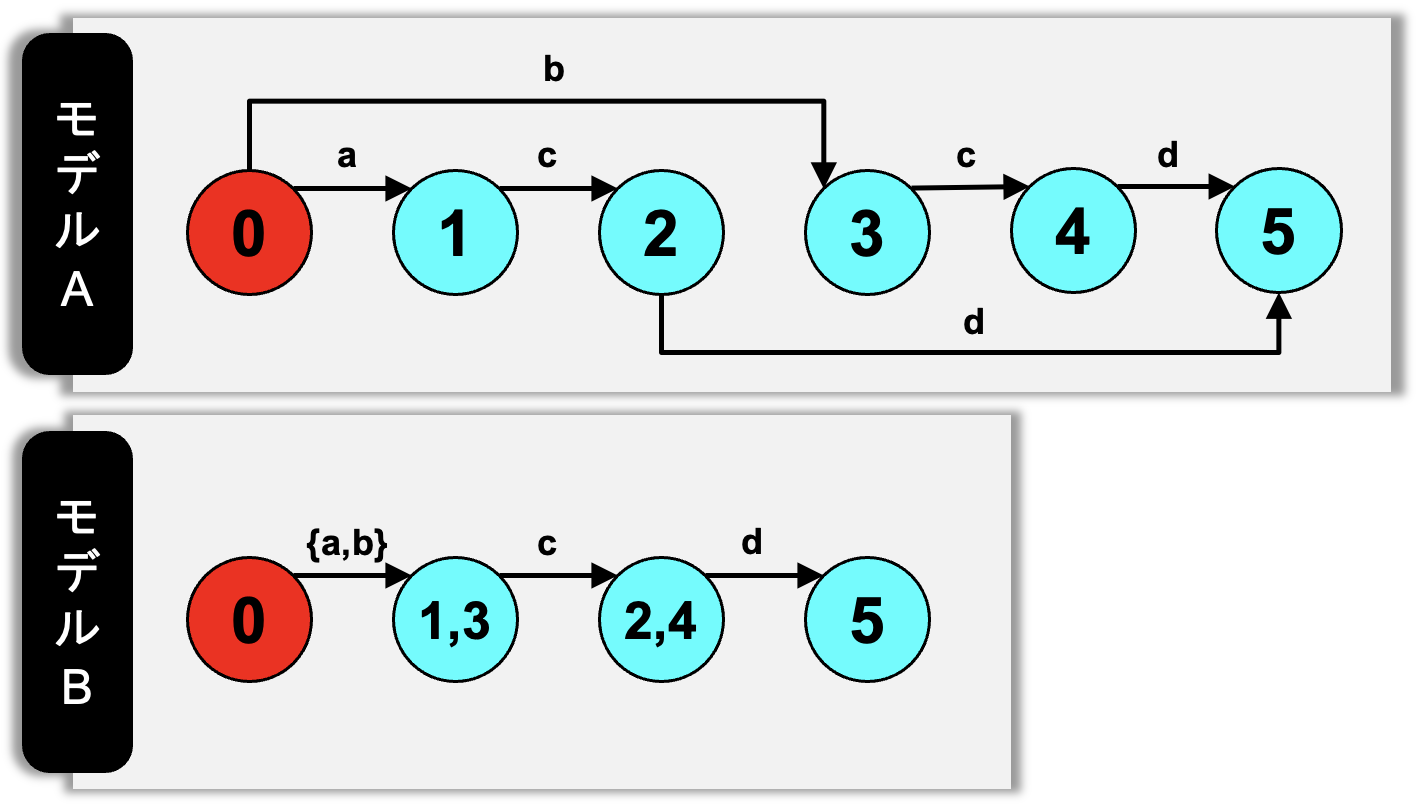
\includegraphics[width=6.3cm]{./figures/minimise.png}
  \caption{LTSの最小化}
  \label{fig:1}
\end{figure}\\
\indent
図\ref{fig:1}にはモデルAとモデルBと名付けられた二つのLTSが示されている．この時，二つのLTSは全く同じ挙動を表し，初期状態0から$a \rightarrow c \rightarrow d$，もしくは$b \rightarrow c \rightarrow d$と遷移することで，状態5に到達する．
このとき，モデルAとモデルBは離散制御器合成を行うにあたって等価なLTSとされ，このLTSの等価性に基づけば，状態数6のモデルAを状態数4のモデルBに変換し，LTSを最小化することができる．
\section{段階的なLTSの最小化を用いた制御器合成}
本研究では，段階的制御器合成の部分合成の各段階においてLTSの等価性に基づきLTSとして表された制御器を最小化する方法を提案し，計算空間の削減を図る．\\
\indent
% LTSの等価性に基づいたLTSの最小化\cite{bisimulation}は，等価なLTSのうち状態数が最小となるLTSを選択することで実現ができる．例えば，以下のような例が考えられる．
% \begin{figure}[htbp]
%   \centering
%   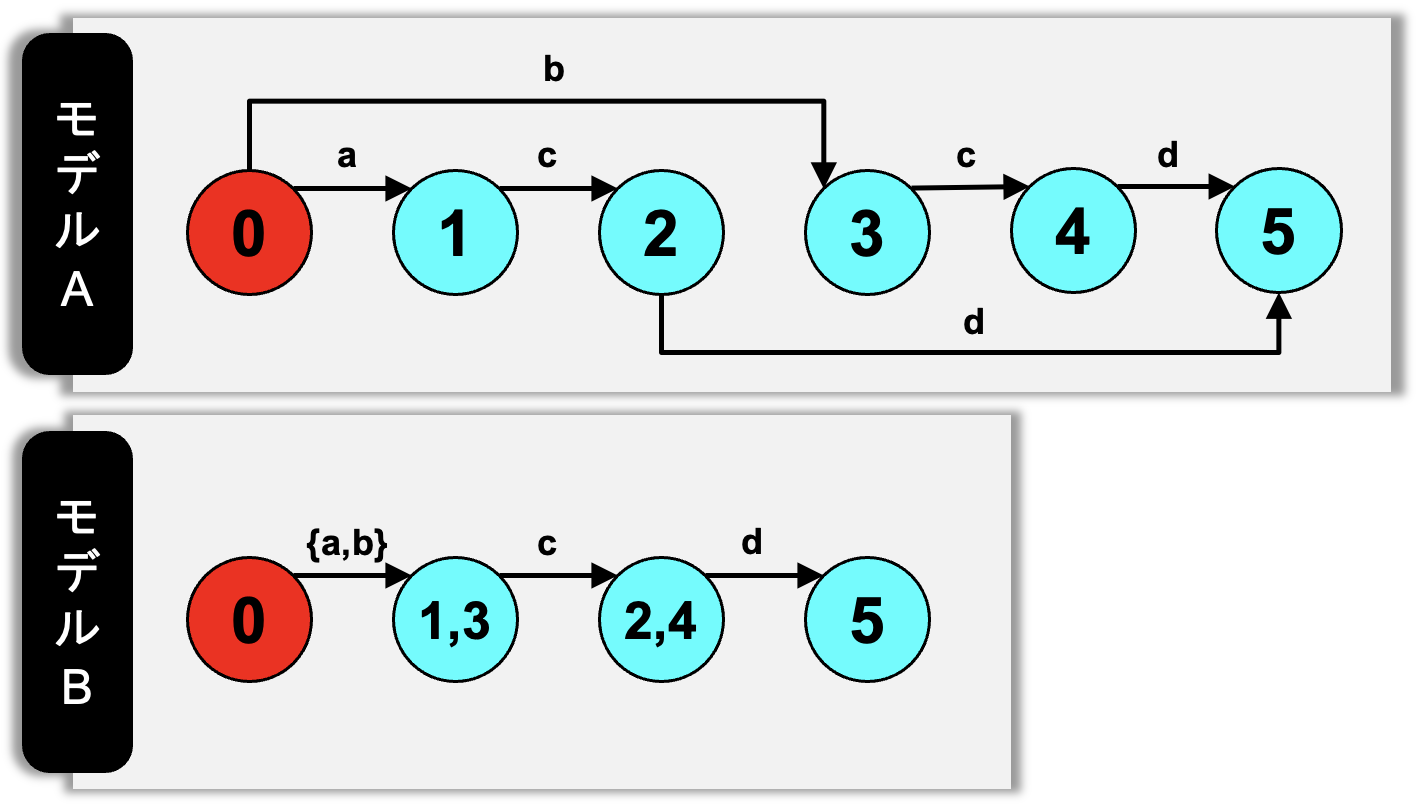
\includegraphics[width=6.3cm]{./figures/minimise.png}
%   \caption{LTSの最小化}
%   \label{fig:1}
% \end{figure}\\
% \indent
% 図\ref{fig:1}にはモデルAとモデルBと名付けられた二つのLTSが示されている．この時，二つのLTSは全く同じ挙動を表し，初期状態0から$a \rightarrow c \rightarrow d$，もしくは$b \rightarrow c \rightarrow d$と遷移することで，状態5に到達する．
% このとき，モデルAとモデルBは離散制御器合成を行うにあたって等価なLTSとされ，このLTSの等価性に基づけば，状態数6のモデルAを状態数4のモデルBに変換し，LTSを最小化することができる．\\
% \indent
段階的制御器合成の部分合成で合成されたLTSに対して最小化を適用し，最小化で削減された状態を以降の部分合成で構築回避する．これにより，最大となる計算空間の状態数を段階的離散制御器合成からさらに削減する．このアルゴリズムはAlgorithm \ref{algorithm:SDCS_mimimise}で表される．
\begin{algorithm}[t]
  \caption{LTSの最小化をする段階的離散制御器合成}
  \label{algorithm:SDCS_mimimise}
  \begin{algorithmic}[1]
  \renewcommand{\algorithmicrequire}{\textbf{Input:}}
  \renewcommand{\algorithmicensure}{\textbf{Output:}}
  \REQUIRE $E$ {\bf such that} $\forall e \in E, e = \{S_{e}, A_{e}, \Delta_{e}, s^0_{e}\}$
  \REQUIRE $R$ {\bf such that} $\forall r \in R, e = \{S_{r}, A_{r}, \Delta_{r}, s^0_{r}\}$
  \ENSURE  $c$
  
  \FOR{$R \neq \emptyset$}
    \STATE $r^* \Leftarrow $ {\bf Stepwise Policy($E,R$)}
    \STATE $E^* \Leftarrow \{\forall e \in E \mid A_e \cap A_{r^*} \neq \emptyset\}$
    \STATE $e^* \Leftarrow $ {\bf Two-Players Game Solver($r^*,E^*$)}
    \STATE $e^* \Leftarrow $ {\bf LTS minimizing($e^*$)}
    % \STATE $g \Leftarrow $ {\bf Game Space Generater($r^*,E^*$)}
    % \STATE $e^* \Leftarrow $ {\bf Two-Players Game Solver($g$)}
    % \STATE $e^* \Leftarrow $ {\bf Discrete Contorller Synthesis($r^*,E^*$)}
    % \STATE $R = $ {\bf Remove Inactive-Transit$R$ $\backslash \{r^*\}$
    % \STATE $E = $ {\bf Remove Inactive-Transitions($E$)} $\backslash E^* \cup \{e^*\}$
    \STATE $R \Leftarrow R \backslash \{r^*\}$
    \STATE $E \Leftarrow E \backslash E^* \cup \{e^*\}$
  \ENDFOR
  \STATE {\bf return} $c \Leftarrow e \in E$
  \end{algorithmic}
  \end{algorithm}

  Algorithm \ref{algorithm:SDCS_mimimise}ではAlgorithm \ref{algorithm:SDCS}（段階的制御器合成のアルゴリズム） の2人プレイヤーゲームを解いた（4行目）あとに，これによって合成された制御器$e^*$をLTSの等価性に基づいた最小化を行う（5行目）．

%\newpage
\section{評価}
本論文では，段階的離散制御器合成にLTSの最小化を適用した事の有用性を確認するために，以下の課題を設定して評価実験を行なった．
\begin{itemize}
  \item 課題1「段階的離散制御器合成にLTSの最小化を適用した場合としない場合で，状態数，遷移数がどれほど削減されるか．」
  \item 課題2「段階的離散制御器合成にLTSの最小化を適用した場合としない場合で，主記憶量，計算時間がどれほど削減されるか．」
\end{itemize}

\indent
本論文での評価に用いるシステムは，ヘッドカウント制御システム\cite{ArtGallery}と自動倉庫管理システム\cite{KIVA}である．ここで，ヘッドカウント制御システムとは，部屋への入室を許可または拒否することで部屋の人数を管理するシステムであり，自動倉庫管理システムとは，倉庫内でロボットが棚を作業者のもとへ運搬することで，商品の取り出しや在庫管理を行うシステムである．また，実験にはOSがWindows 11 Pro，CPUがIntel Core Ultra 9 285K，RAMが128GB (DDR5-4400)の計算機を使用し，MTSA\cite{MTSA}を用いて制御器の合成を実施した．その結果が表\ref{table:evaluation_artgallery_kiva_final_data}である．また，表\ref{table:evaluation_artgallery_kiva_final_data}中の削減率は，最小化なしの手法から，最小化ありの手法の値がどれだけ削減されたかを表す．


\begin{table}[t]
  \caption{制御器の合成に必要となった状態数，遷移数，主記憶量(MB)，計算時間(s)}
  \label{table:evaluation_artgallery_kiva_final_data}
  \begin{center}
  \begin{tabular}{ccc|rr|rr}
  \toprule
  \multicolumn{3}{c|}{} & \multicolumn{2}{c|}{部屋の数=5} & \multicolumn{2}{c}{部屋の数=6} \\
  \multicolumn{3}{c|}{} & \multicolumn{1}{c}{値} & \multicolumn{1}{c|}{削減率(\%)} & \multicolumn{1}{c}{値} & \multicolumn{1}{c}{削減率(\%)} \\
  \hline
  \multirow{8}{*}{\rotatebox[origin=c]{90}{ヘッドカウント制御}}
  & \multirow{4}{*}{\rotatebox[origin=c]{90}{最小化なし}}
  & 状態数 & 15,725 & - & 60,131 & - \\
  & & 遷移数 & 27,814 & - & 106,816 & - \\
  & & 主記憶量(MB) & 124.92 & - & 375.58 & - \\
  & & 計算時間(s) & 3.305 & - & 7.194 & - \\
  \cline{2-7}
  & \multirow{4}{*}{\rotatebox[origin=c]{90}{最小化あり}}
  & 状態数 & 12,350 & -21.5 & 36,172 & -23.2 \\
  & & 遷移数 & 22,603 & -18.7 & 84,865 & -20.6 \\
  & & 主記憶量(MB) & 126.99 & +1.7 & 538.25 & +43.3 \\
  & & 計算時間(s) & 4.507 & +36.4 & 34.746 & +383.0 \\
  \hline
  \multicolumn{3}{c|}{} & \multicolumn{2}{c|}{ロボットの数=3} & \multicolumn{2}{c}{ロボットの数=4} \\
  \multicolumn{3}{c|}{} & \multicolumn{1}{c}{値} & \multicolumn{1}{c|}{削減率(\%)} & \multicolumn{1}{c}{値} & \multicolumn{1}{c}{削減率(\%)} \\
  \hline
  \multirow{8}{*}{\rotatebox[origin=c]{90}{自動倉庫}}
  & \multirow{4}{*}{\rotatebox[origin=c]{90}{最小化なし}}
  & 状態数 & 489,212 & - & 670,320 & - \\
  & & 遷移数 & 2,100,488 & - & 3,000,732 & - \\
  & & 主記憶量(MB) & 4,183.17 & - & 6,254.61 & - \\
  & & 計算時間(s) & 39.362 & - & 97.718 & - \\
  \cline{2-7}
  & \multirow{4}{*}{\rotatebox[origin=c]{90}{最小化あり}}
  & 状態数 & 115,348 & -76.4 & 228,228 & -66.0 \\
  & & 遷移数 & 506,768 & -75.9 & 1,006,985 & -66.4 \\
  & & 主記憶量(MB) & 1,081.77 & -74.1 & 2,144.75 & -65.7 \\
  & & 計算時間(s) & 34.119 & -13.3 & 23.701 & -75.7 \\
  \bottomrule
  \end{tabular}
  \end{center}
\end{table}

表\ref{table:evaluation_artgallery_kiva_final_data}を見ると，ヘッドカウント制御では状態数が平均22.4\%，遷移数が平均19.7\%，自動倉庫システムでは状態数が平均71.2\%，遷移数が平均71.2\%削減されていることがわかる．また，主記憶量と計算時間については，ヘッドカウント制御では主記憶量が平均22.5\%，計算時間が平均209.7\%増加し，自動倉庫では主記憶量が平均69.9\%，計算時間が平均44.5\%減少していることがわかる．\\
\indent
以上の結果から，課題1に関しては，両システムともに状態数と遷移数が削減されており，LTSの最小化が計算空間の削減に寄与していることがわかった．一方，課題2に関しては，主記憶量と計算時間については，ヘッドカウント制御では増加，自動倉庫では減少しており，一概にLTSの最小化が主記憶量と計算時間の削減に寄与しているとは言えなかった．


\section{おわりに}
本論文では，離散制御器合成における計算空間爆発に対処するため，LTSの等価性を考慮した離散制御器合成の計算空間削減に取り組んだ．段階的制御器合成の各段階で合成されたLTSに対して最小化を適用し，最小化で削減された状態を以降の部分合成で構築回避することで，最大となる計算空間の状態数を段階的離散制御器合成からさらに削減する手法を提案した．評価実験では，ヘッドカウント制御と自動倉庫のシステム両方で，状態数と遷移数が削減されていることがわかり，LTSの最小化が計算空間の削減に寄与していることがわかった．しかし，主記憶量と計算時間については，ヘッドカウント制御では増加，自動倉庫では減少しており，一概にLTSの最小化が主記憶量と計算時間の削減に寄与しているとは言えなかった．\\
\indent
本論文では，部分合成の各段階の最後にLTSの最小化を挟んだが，今後は，LTS の最小化を全段階ではなく，特定の段階にのみ適用する方法を検討する．これによって，本手法の限界である主記憶量と計算時間の増加への対処を目指す．


\newpage

\begin{thebibliography}{99} % 文献リスト一覧はこんな風に始める
  {\footnotesize
  
  \bibitem{rebok}
  要求工学知識体系 REBOK: Requirements Engineering Body Of Knowledge, 第1版, 2011, 近代科学社
  
  \bibitem{concurrency}
  J.~Magee and J.~Kramer, 
  {\it Concurrency: State Models and Java Programs}, 2006.
  \bibitem{LTS}
  C. Baier and J.-P. Katoen, Principles of Model Checking, The MIT Press, 2008.

  \bibitem{Thuijsman2020}
  S.~B.~Thuijsman and M.~A.~Reniers, ``Transformational Supervisor Synthesis for Evolving Systems,'' {\it IFAC-PapersOnLine}, vol.~53, no.~4, pp.~309--316, 2020.
  
  \bibitem{yamauchi} 
  山内拓人, 鄭顕志, 段階的な部分合成による離散制御器合成の分析空間削減, 
  IEICE, Vol.~J106-D, No.~4, pp.~218--230, 2023.

  \bibitem{bisimulation}
  Flordal H, Malik R, Fabian M, Akesson K.: Compositional synthesis of maximally permissive supervisors using supervision equivalence. Discret Event Dynamic Systems, Vol 17, pp. 475–504, 2007. https://doi.org/10.1007/s10626-007-0018-z

  \bibitem{ArtGallery}
  A. Borda, L. Pasquale, V. Koutavas, and B. Nuseibeh, “Compositional verification of self-adaptive cyber-physical systems,” 2018IEEE/ACM 13th International Symposium on Software Engineeringfor Adaptive and Self-Managing Systems, pp.1–11, 2018.

  \bibitem{KIVA}
  J. Enright and P.R. Wurman, “Optimization and coordinated au-tonomy in mobile fulfillment systems,” Automated Action Plan-ning for Autonomous Mobile Robots, 2011 AAAI Workshop, SanFrancisco, California, USA, August 7, 2011, pp.33–38, 2011.
  http://www.aaai.org/ocs/index.php/WS/AAAIW11/paper/view/3917

  \bibitem{MTSA}
  N. D’Ippolito, D. Fischbein, M. Chechik, and S. Uchitel,“MTSA: the modal transition system analyser,” 23rd IEEE/ACMInternational Conference on Automated Software Engineering,15-19 September 2008, L’Aquila, Italy, pp.475–476, 2008.
  https://doi.org/10.1109/ASE.2008.78
  
  }
  \end{thebibliography} % 文献リストの最後に必要

\end{document}
